%TODO
%	Procurar protocolos de gerencia especificos pra IoT
%
%	Capitulo de Gerencia de Redes com um viés mais IoT.
%
%	Na parte de gerência justificar a escolha do snmp por ser um padrão e 
% argumentar que é importante usá-lo para aproveitar a infraestrutura já 
% existente.
%
%	Comparar os protocolos de gerencia especificos pra IoT e dar enfase aos 
% pros e contras de cada um e entrar com a minha proposta pra melhorar esses 
% pontos.
%
%=======================================================================
% Declarações iniciais identificando a classe de documento e
% selecionando alguns pacotes adicionais.
%
% As opções disponíveis (separe-as com vírgulas, sem espaço) são:
% - twoside: Formata o documento para impressão frente-e-verso
%   (o default é somente-frente)
% - english,brazilian,french,german,etc.: idiomas usados no documento.
%   Deve ser colocado por último o idioma principal.
%=======================================================================
\documentclass[twoside,english,brazilian]{UNISINOSmonografia}
\usepackage[utf8]{inputenc} % charset do texto (utf8, latin1, etc.)
\usepackage[T1]{fontenc} % encoding da fonte (afeta a sep. de sílabas)
\usepackage{graphicx} % comandos para gráficos e inclusão de figuras

\usepackage{bibentry} % para inserir refs. bib. no meio do texto
\usepackage{hyperref}



\hypersetup{
	breaklinks=true,
	unicode=true,          % non-Latin characters in Acrobat’s bookmarks
	hidelinks=true,
	linktoc=all,
	pdflang=pt-BR
}

\graphicspath{ {./images/} }

%\hypersetup{
%	pdftitle={titulo},    % title
%	pdfauthor={mateus},     % author
%	pdfsubject={subsubsub},   % subject of the document
%	pdfkeywords={kkk1} {key2} {key3}, % list of keywords
%}
%=======================================================================
% Escolha do sistema para geração de referências bibliográficas.
%
% O default é usar o estilo unisinos.bst.  Comente a definição abaixo
% e descomente a linha seguinte para usar o estilo do ABNTeX (é
% necessário ter esse pacote instalado).
%
% A vantagem do unisinos.bst é que ele permite o uso de um arquivo .bib
% seguindo as orientações tradicionais do BibTeX (veja essas orientações
% em http://ctan.tug.org/tex-archive/biblio/bibtex/contrib/doc/btxdoc.pdf).
% Entretanto, o estilo não suporta algumas citações mais exóticas como
% apud.  Para isso, use o ABNTeX, mas esteja ciente de que muitas de
% suas referências serão incompatíveis com os estilos tradicionais do
% BibTeX como plain, alpha, ieeetr, entre outros.
%=======================================================================
\unisinosbst
%\usepackage[alf]{abntcite}



%=======================================================================
% Dados gerais sobre o trabalho.
%=======================================================================
\autor{Aubin}{Mateus Rauback}
\author{Mateus Rauback Aubin}
\titulo{
Um Sistema de Gestão de Dispositivos Inteligentes 
Baseado em Protocolos de Gerência de Redes Voltado Para a 
Internet das Coisas
}
%\subtitulo{Versão \LaTeX}
\orientador[Prof.~Dr.]{Ávila}{Rafael Bohrer}
%\coorientador[Prof.~Dr.]{Lamport}{Leslie}
\local{São Leopoldo}
\ano{2013}

%% dados específicos para monografia de Graduação
\unidade{Unidade Acadêmica Graduação}
\curso{Curso de Bacharelado em Ciência da Computação}
\natureza{
Trabalho de Conclusão de Curso apresentado como requisito parcial
para a obtenção do título de Bacharel em Ciência da Computação
pela Universidade do Vale do Rio dos Sinos --- Unisinos
}


%=======================================================================
% Palavras Chave.
%
% Deve ser fornecida para cada idioma.
%=======================================================================
\palavrachave{brazilian}{Internet das Coisas}
\palavrachave{english}{Internet of Things}

\palavrachave{brazilian}{Gerência de Redes}
\palavrachave{english}{Network Management}

\palavrachave{brazilian}{Protocolos de Rede}
\palavrachave{english}{Network Protocols}


%=======================================================================
% Início do documento.
%=======================================================================
\begin{document}	
\capa
\folhaderosto

%=======================================================================
% Dedicatória (opcional).
%
% O texto é normalmente colocado na parte de baixo da página, alinhado
% à direita.  Mas a formatação é basicamente livre.  Só não se escreve
% a palavra 'dedicatória'.
%=======================================================================
%\begin{dedicatoria}
%Aos nossos pais.\\[4ex] % quebra a linha dando um espaçamento maior
%\begin{itshape} % faz o texto ficar em itálico
%If I have seen farther than others,\\
%it is because I stood on the shoulders of giants.\\
%\end{itshape}
%--- \textsc{Sir Isaac Newton} % \textsc é o "small caps"
%\end{dedicatoria}


%=======================================================================
% Agradecimentos (opcional).
%=======================================================================
%\begin{agradecimentos}
%Obrigado!
%\end{agradecimentos}


%=======================================================================
% Epígrafe (opcional).
%
% ``[...] o autor apresenta uma citação, seguida de indicação de autoria,
% relacionada com a matéria tratada no corpo do trabalho. Podem, também,
% constar epígrafes nas folhas de aberturas das seções primárias.''
%=======================================================================
%\begin{epigrafe}
%``\textit{Ninguém abre um livro sem que aprenda alguma coisa}''.\\
%(Anônimo)
%\end{epigrafe}


%=======================================================================
% Resumo em Português.
%
% A recomendação é para 150 a 500 palavras.
%=======================================================================
%\begin{abstract}
%	Dica para elaborar um bom resumo: ele tem que responder às seguintes 
%questões:
%	- o que? (contexto)
%	- por que? (motivação)
%	- para que? (objetivos)
%	- como? (metodologia)
%\end{abstract}


%=======================================================================
% Resumo em língua estrangeira (obrigatório somente para teses e
% dissertações).
%
% O idioma usado aqui deve necessariamente aparecer nos parâmetros do
% \documentclass, no início do documento.
%=======================================================================
%\begin{otherlanguage}{english}
%\begin{abstract}
%Abstract goes here
%\end{abstract}
%\end{otherlanguage}


%=======================================================================
% Lista de Figuras (opcional).
%=======================================================================
%\listoffigures


%=======================================================================
% Lista de Tabelas (opcional).
%=======================================================================
%\listoftables


%=======================================================================
% Lista de Abreviaturas (opcional).
%
% Deve ser passada como parâmetro a maior das abreviaturas utilizadas.
%=======================================================================
%\begin{listadeabreviaturas}{seg., segs.}
%\item[ampl.] ampliado, -a
%\item[atual.] atualizado, -a
%\item[coord.] coordenador
%\item[N.~T.] Novo Testamento
%\item[seg., segs.] seguinte, -s
%\end{listadeabreviaturas}


%=======================================================================
% Lista de Siglas (opcional).
%
% Deve ser passada como parâmetro a maior das siglas utilizadas.
%=======================================================================
\begin{listadesiglas}{SNMP}
\item[IoT] Internet of Things
\item[M2M] Machine-To-Machine
\item[TI] Tecnologia da Informação
\item[TCP] Transmission Control Protocol
\item[IP] Internet Protocol
\item[IPv6] Internet Protocol version 6
\item[SLA] Service Level Agreement
\item[CMIP] Common Management Information Protocol
\item[IETF] Internet Engineering Task Force
\item[SNMP] Simple Network Management Protocol
\item[RFC] Request For Comments
\item[SMI] Structure of Management Information
\item[MIB] Management Information Base
%\item[CAPES] Coordenação de Aperfeiçoamento de Pessoal de Nível Superior
%\item[FAPERGS] Fundação de Amparo à Pesquisa do Estado do Rio Grande do Sul
\end{listadesiglas}


%=======================================================================
% Lista de Símbolos (opcional).
%
% Deve ser passado o maior (mais largo) dos símbolos utilizados.
%=======================================================================
%\begin{listadesimbolos}{Ca}
%\item[\textsuperscript{o}C] Graus Celsius
%\item[Al] Alumínio
%\item[Ca] Cálcio
%\end{listadesimbolos}


%=======================================================================
% Sumário
%=======================================================================
\tableofcontents


%=======================================================================
% Introdução
%=======================================================================
\chapter{Introdução}

% as epígrafes nos capítulos são opcionais
\epigrafecap{
	In the nineteenth century, machines learned to do; in the twentieth 
	century, they learned to think; and in the twenty-first century, they are 
	learning to perceive -- they actually sense and respond.
}{\citetexto{Sundmaeker2010}}

%	Deve conter:
%		Apresentação do Assunto: IoT
%		Delimitação do Assunto:  Gerência de Redes aplicada a IoT
%		Justificativa:           Porque vai mudar a vida cotidiana
%		Localizar no Tempo:      Trabalhos de IoT
%		Ressaltar a Importância: Igual justificativa
%		Apresentar Objetivos:    Vide proposta
%		Apresentar a Estrutura:  Fica pro final
%		Explicar a Metodologia:  Vai ter capítulo específico

	Desde a Revolução Industrial há uma crescente busca pela automação das 
	tarefas humanas. Através de máquinas cada vez mais sofisticadas foi 
	possível obter significativo avanço nas tecnologias e nos métodos de 
	produção ao passo que diversas tarefas deixaram de ser realizadas 
	manualmente.
	Seguindo esta filosofia, máquinas computacionais foram projetadas e as 
	bases da ciência da computação estabelecidas. Conceitos como a 
	Álgebra Booleana de \citetexto{boole2003}, publicado originalmente em 
	1854, servem até hoje como fundamentos deste campo de estudos.

	Durante a segunda guerra mundial houve um expressivo progresso na 
	computação graças ao incentivo das organizações de defesa para melhorar 
	métodos de cálculo e criptografia. Neste período publicações como as de 
	\citetexto{Shannon1948}, \citetexto{Turing1937} e 
	\citetexto{VonNeumann1945} definiram a ciência da computação como é 
	conhecida hoje.

	Ainda com objetivos de defesa, pesquisas no campo de redes de computadores 
	começaram a ser desenvolvidas nos anos que seguiram. A IBM, nos anos 50,
	desenvolveu para os EUA o SAGE\footnote{Semi-Automatic Ground Environment, 
	um sistema nacional de defesa do espaço aéreo e um dos mais importantes 
	projetos da IBM. 
	\urlbr{set.~2013}{www.ibm.com/ibm/history/ibm100/us/en/icons/sage/}}, 
	um dos primeiros exemplos de computadores conectados em rede, 
	caracterizado pela ``transmissão de dados digitais em linhas telefônicas 
	de voz à 1300 bits por segundo'' \cite{IBMSAGE1983}.

	Contudo, o SAGE comunicava-se através do conceito de circuitos, que, mais 
	tarde, mostrou-se inferior à troca de pacotes (\textit{packet switching}). 
	Explorado pela agência de defesa americana nos anos 70, a comunicação via 
	troca de pacotes originou a ARPANET, uma rede nacional descentralizada 
	utilizada para interligar universidades e centros de pesquisas 
	\cite{ARPANET1964}, assim como os protocolos TCP/IP, a base da atual 
	internet.

	A contínua ampliação da capacidade de processamento dos dispositivos 
	computacionais, aliada a redução de custos, possibilitou uma nova 
	revolução tecnológica \cite{Atzori2010b}, abrindo caminho para a Era da 
	Informação.
	Munidos de circuitos integrados e \textit{microchips}, os computadores 
	estão cada vez mais presentes nas atividades humanas, avançando em direção 
	à ubiquidade.
	
	No atual cenário tecnológico já é possível, de maneira economicamente 
	viável, colocar em prática algumas das ideias vislumbradas por 
	\citetexto{Weiser1991}. 
	Apesar de representar um desafio para diversas áreas do conhecimento, as 
	barreiras para a efetiva integração entre dispositivos computacionais e a 
	vida cotidiana têm diminuído, possibilitando a criação de novos produtos e 
	serviços, resultando em soluções para os mais diversos problemas.
	
	Ainda que não seja uma proposta nova, \citetexto{Turck2013} pontua que a 
	implementação de uma rede composta de dispositivos embarcados em objetos 
	do dia-a-dia, ou seja, a Internet das Coisas (IoT), não era viável devido 
	a fatores como complexidade e custo. 
	Entretanto, tomando por referência a lei de \citetexto{Moore1965}, a qual 
	dita que o número de transístores em um circuito integrado dobra 
	aproximadamente a cada dois anos, é improvável que se reverta a tendência 
	de dispositivos cada vez menores e mais baratos, se reverta.
	
	Diversas são as semelhanças entre a Internet das Coisas e as Redes de 
	Sensores sem Fio, porém, enquanto as redes de sensores  
	são implantadas principalmente com o intuito de monitorar variáveis em um 
	ambiente \cite{Sakthidharan2012}, a Internet das Coisas expande este 
	conceito ao próximo nível. 
	A capacidade de tornar cada dispositivo individualmente endereçável na 
	internet favorece o compartilhamento de informações entre sistemas, 
	resultando em uma modalidade de comunicação chamada pela 
	\citetexto{ETSI2010} de comunicação Máquina-a-Máquina (M2M).
	
	Motivados pelas oportunidades e pelo alto impacto social da computação 
	pervasiva, impulsionada com a ajuda da IoT, pesquisadores tanto da 
	academia quanto da indústria se mobilizaram em torno deste conceito 
	\cite{Atzori2010b}. 
	Entidades governamentais reconheceram também a IoT como um paradigma 
	promissor, fomentando iniciativas de pesquisa e desenvolvimento em países 
	como China, Japão, Estados Unidos e da União Europeia 
	% p 16
	\cite{Sundmaeker2010}.
	
	Entretanto, com grandes poderes vêm grandes responsabilidades
	\footnote{Lição dada a Peter Parker por seu tio Ben na história em 
	quadrinhos Homem-Aranha, escrita por Stan Lee.}. 
	Para realizar sua visão, a Internet das Coisas deve superar uma série de 
	desafios, entre eles: privacidade, padronização tecnológica e 
	escalabilidade \cite{Coetzee2011}. 
	Para tanto, a cooperação entre academia, indústria e governo é fundamental 
	para que a IoT possa demonstrar seu verdadeiro potencial.
	
%TODO Apresentar a estrutura do trabalho (no cap x falaremos de IoT, no cap Y 
%		de Gerência, tal tal e tal)

\section{Justificativa e Definição do Problema}
%	Abordar
%		Justificativa: Porque com um monte de dispositivos espalhados por aí 
%		               vai ser difícil gerenciá-los um a um
%		Problema: Como fazer isso remotamente? Como fazer isso de maneira 
%		          padronizada? Como reaproveitar tecnologias estabelecidas?
%		Objetivo: Para facilitar a gestão de dispositivos inteligentes

	Em um mundo cada vez mais conectado e dependente da internet, a quantidade 
	de dispositivos capazes de integrar a rede já representa uma fatia 
	considerável entre os aparelhos usados diariamente \cite{Accenture2012}.
	Computadores, \textit{laptops}, \textit{tablets}, \textit{smartphones} e 
	televisores integram uma crescente classe de produtos comercialmente 
	chamados de Dispositivos Inteligentes (\textit{Smart Devices}) e que 
	permitem, dentre outras funções, acesso a redes e, consequentemente, à 
	internet.
	
	Paralelamente a esta tendência e seguindo as previsões de 
	\citetexto{Gilder2007} e \citetexto{Moore1965}, por exemplo, a capacidade 
	de equipamentos e redes continua a aumentar, resultando na visão de um 
	atraente e economicamente viável mundo conectado \cite{Ding2009}.
	Tais mudanças influenciam direta e indiretamente a sociedade, seus 
	costumes, e, conforme afirma \citetexto{Carr2010}, até mesmo o pensamento 
	humano.
	
	A difusão de aparelhos capazes de acessar a internet criou um novo 
	paradigma que está transformando a gestão de Tecnologia da Informação (TI) 
	\cite{ZdnetBYOD}.
	Este aumento apresenta-se como um desafio para as áreas de segurança da 
	informação e gerência de redes, convidando grandes empresas como 
	\citetexto{CiscoBYOD}, \citetexto{HP2013} e \citetexto{Motorola2011} a 
	propor novas soluções.
	
	Apesar de constituir um desafio de gestão, não há indícios da redução de 
	dispositivos nas redes. A Internet das Coisas trará consigo uma vasta gama 
	de novos aparelhos que carecem de diretivas de gestão \cite{Atzori2010b} 
	e, ainda que novas soluções estejam em desenvolvimento, não há um acordo 
	sobre mecanismos específicos de gerência, resultando em soluções 
	proprietárias e que não colaboram entre si.
	
	Visando manter a interoperabilidade entre dispositivos, há, nas pesquisas 
	de IoT, um consenso referente ao uso do Protocolo de Internet (IP), mais 
	especificamente o IPv6, como o protocolo padrão de comunicação 
	\cite{Dunkels2008,Mattern2010a,Feng2011,Paventhan2012}.
	Compartilhando desta motivação, autores como \citetexto{Sundmaeker2010}, 
	\citetexto{Mattern2010a} e \citetexto{Wang2012}
	afirmam que os protocolos de gerenciamento de redes devem, também, manter 
	a compatibilidade com os padrões já existentes, sendo, se necessário, 
	estendidos para dar suporte aos desafios da IoT.
	
	Para tanto, é de grande interesse da indústria e da academia que um 
	protocolo de gerência de redes possa desempenhar seu papel em conjunto com 
	a infraestrutura já existente sem deixar de atender às restrições e 
	características da IoT. É nesta tarefa que concentram-se os esforços deste 
	trabalho, buscando melhorias específicas para este novo cenário e, ao 
	mesmo tempo, manter a interoperabilidade com padrões já estabelecidos.
	
\section{Objetivos}

	Corroborando a visão apresentada, o presente trabalho se propõe a estudar 
	e 
	criar mecanismos que possibilitem o emprego de protocolos e modelos da 
	gerência de redes tradicional aplicados ao contexto de Internet das 
	Coisas. 
	
	Os dispositivos embarcados\footnote{
Tais dispositivos são caracterizados pela escassez de recursos computacionais 
e que atuam de forma praticamente autônoma, requerindo pouca ou nenhuma 
configuração.
%TODO adicionar citação
	}
	que compõem a Internet das Coisas não contam 
	com interfaces de usuário, causando com que toda sua gestão deva ser 
	realizada remotamente ou de forma automatizada. Enquanto, idealmente, um 
	dispositivo deveria ser auto-gerenciável, é improvável que tais métodos 
	sejam apropriados ou até mesmo possíveis em todas as situações. Desta 
	forma, eventualmente será 
	necessária a intervenção manual sobre um ou mais destes dispositivos.

	Devido a ausência de padrões de gerenciamento para IoT é provável que cada 
	fabricante 
	proponha diferentes maneiras de realizar esta gestão, criando 
	implementações 
	incompatíveis e de padrão fechado. Esta filosofia vai diretamente 
	de encontro a mentalidade da Internet, que é composta por padrões livres e 
	abertos,
	para que todos (indivíduos e organizações) tenham acesso.

	Porém, a gestão da Internet das Coisas apresenta características únicas 
	não contempladas pelos padrões já estabelecidos, entre elas estão a grande 
	quantidade de dispositivos presentes na rede e a reduzida capacidade de 
	processamento. Surge, então, a necessidade de estudar e ajustar estes 
	protocolos para este contexto, de forma que atendam às necessidades da IoT.

	Uma vez encontradas as fraquezas da gerência de redes tradicional no 
	contexto de IoT, este trabalho apresentará sugestões de melhorias ao 
	processo de gestão.
	Tais funcionalidades devem, idealmente, manter a compatibilidade com o 
	protocolo, funcionando como extensões. 
	O resultado final deve conter o detalhamento das melhorias propostas e uma 
	implementação das mesmas, realizada a título de prova de conceito.

\subsection{Objetivo Geral}

Projetar e implementar uma solução que permita o uso de modelos da gerência de 
redes tradicional (protocolos e sistemas) para gerir dispositivos em um 
contexto de Internet das Coisas.

\subsection{Objetivos Específicos}

	\begin{itemize}
		\item 
		Aprofundar os conhecimentos sobre protocolos de Gerência de 
		Redes e sobre protocolos utilizados por dispositivos aplicados 
		à Internet das Coisas;
		
		\item
		Projetar uma solução que possibilite o uso de ferramentas e protocolos 
		da gerência de redes tradicional no contexto de IoT;
		
		\item
		Desenvolver um protótipo da solução projetada como prova de conceito;

		\item
		Avaliar a solução em termos de suas forças, fraquezas e futuras 
		oportunidades.
		
	\end{itemize}


\section{Método de Pesquisa}

Para atingir seus objetivos, a presente pesquisa é caracterizada por uma 
abordagem quantitativa 
``que tem suas raízes no pensamento positivista lógico, tende a enfatizar o 
raciocínio dedutivo, as regras da lógica e os atributos mensuráveis''
\cite{Gerhardt2009},
e busca
``traduzir em números opiniões e informações para classificá-las e 
analisá-las''
\cite{MetodologiaUFSC2005}.
Ao estabelecer como contexto as áreas de Gerência de Redes e Internet das 
Coisas, atribui-se a natureza de pesquisa aplicada, onde os resultados serão 
adequados para a
``aplicação prática e dirigidos à solução de problemas específicos''
\cite{MetodologiaUFSC2005}.

Quanto aos seus procedimentos técnicos, esta será uma pesquisa experimental. 
Neste aspecto, \citetexto{MetodologiaUFSC2005} e \citetexto{Gerhardt2009} 
apoiam-se em \citetexto{Gil2007}, que a define como o processo de determinar um 
objeto de estudo, selecionar variáveis capazes de influenciá-lo e definir 
formas de controle e observação destas variáveis.
Um maior detalhamento, segundo \citetexto{Fonseca2002}, ainda é possível, onde 
deve-se dividir a pesquisa experimental em duas categorias, a de campo e a de 
laboratório, realizada neste trabalho.

Desta forma, pode-se classificar o presente trabalho como uma proposta de 
melhoria na abordagem de gerência de redes. Considerando que ``não é 
necessário, porém, que o autor de algum método novo demonstre que o seu método 
é melhor do que outro método do estado da arte para toda e qualquer situação'' 
\cite{Wazlawick2008} a abrangência do trabalho é intencionalmente limitada ao 
domínio da Internet das Coisas. % no contexto de home-automation?!

Para avaliar a eficácia das melhorias propostas uma implementação a título de  
protótipo será desenvolvida, possibilitando a comparação direta entre 
estratégias já estabelecidas (estado da arte) e a proposta. Caracteriza-se, 
portanto, como uma pesquisa quantitativa que se propõe a ``verificar o
quão melhor é usar um programa/sistema novo frente à(s) alternativa(s)'' 
\cite{Jacques2007}.
Faz-se necessária, então, a escolha de indicadores técnicos que
possibilitem uma avaliação clara e objetiva do desempenho do 
método proposto frente ao estado da arte, são eles:

%TODO Pedir ajuda pro Rafael pra definir os indicadores.

\begin{itemize}
	% http://eprints.eemcs.utwente.nl/7111/01/2004-eTNSM.pdf
	% - Bandwidth usage
	% - CPU time
	% - Memory usage
	% - Round trip delay

	\item Tráfego de Rede: 
Quantidade total de dados trafegados na rede durante uma requisição para N dispositivos.

	\item Tempo de Resposta Total: 
Intervalo de tempo entre a requisição e a obtenção das respostas de todos os dispositivos.

	\item Outros: \dots
\end{itemize}


\chapter{Gerência de Redes}

	Impulsionada pelo crescimento e evolução das redes de computadores, as 
	técnicas de gerência de redes se tornaram fundamentais para garantir o 
	funcionamento e a qualidade dos serviços prestados. Cada vez mais 
	importantes para as atividades humanas, as redes de computadores, em 
	especial a internet, ``têm catalizado a inovação e favorecido a emergência 
	de novos e disruptivos modelos de negócio'' \cite{Ding2009}.
	
	De acordo com \citetexto{Clemm2006}, a gerência de redes pode ser definida 
	como ``as atividades, métodos, procedimentos, e ferramentas que dizem 
	respeito a operação, administração, manutenção e provisionamento de 
	sistemas de rede''. Uma definição extensiva do conceito de gerência de 
	redes é fornecida por \citetexto{Ding2009}:
	
	\begin{quote}
		a execução de um conjunto de funções requeridas para controlar, 
		planejar, alocar, implantar, coordenar, e monitorar os recursos de uma 
		rede de telecomunicações ou de computadores, incluindo a realização de 
		funções como planejamento inicial da rede, atribuição de frequências, 
		roteamento predefinido de tráfico para suportar balanceamento de 
		carga, autorização de distribuição de chaves criptográficas, gerência 
		de configuração, gerenciamento de falhas, gestão da segurança, 
		gerência de performance e gestão de contabilização.~
		\cite[p.~64]{Ding2009}.
% defined as the execution of the set of functions required for 
% controlling, planning, allocating, deploying, coordinating, and 
% monitoring the resources of a telecommunications network or a computer 
% network, including performing functions such as initial network 
% planning, frequency allocation, predetermined traffic routing to 
% support load balancing, cryptographic key distribution authorization, 
% configuration management, fault management, security management, 
% performance management, and accounting management.
	\end{quote}
	
	O reconhecimento da importância das técnicas de gerência de redes provocou 
	esforços por parte de órgãos reguladores, como a Organização Internacional 
	para Padronização (ISO). Em sua normativa 7498-4, a \citetexto{ISO1989} 
	define as cinco principais categorias da gerência de redes, conhecido como 
	o modelo \textbf{FCAPS} que contempla o gerenciamento de:
	
	\begin{itemize}
		% gerenciamento/gerencia/gestao?
		\item \textbf{\textit{Fault} -- Falhas:} 
Engloba todas as ações de detecção e correção de falhas que possam ocorrer na 
rede e em seus equipamentos. 
Segundo \citetexto{Ding2009}, é composta por três passos fundamentais: 
Detecção, Isolamento e Correção. 
Em suma, o ``gerenciamento de falhas está portanto interessado no 
monitoramento da rede para garantir que tudo esteja funcionando regularmente e 
reagir quando este não for o caso'' \cite{Clemm2006}.

		\item \textbf{\textit{Configuration} -- Configuração:}
Responsável por manter uma lista completa e atualizada de todos os ativos que 
compõem a rede, guardando informações como: Configurações de Hardware, Versões 
de Sistemas, Serviços e Documentação.
\cite{Clemm2006,Ding2009,Mauro2009}
A manutenção de tal inventário não é uma tarefa trivial, devendo contemplar a 
inclusão, remoção e atualização de dados sobre cada dispositivo que compõe a 
rede. 
Portanto uma boa gerência de configuração, ``para realizar estas 
atividades deve monitorar todas as mudanças feitas aos recursos'' 
\cite{Wang2012}.

% in order to fulfill these functionalities, 
% it must track all changes made to network resources

		\item \textbf{\textit{Accounting} -- Contabilização:}
Contempla principalmente a coleta de estatísticas sobre usuários e/ou grupos 
de usuários. 
Apontada por \citetexto{Hunt1997} como desejável para o repasse 
de custos do uso de recursos aos usuários, esta categoria é de especial 
importância para empresas pois auxilia na cobrança à clientes internos e 
externos \cite{Clemm2006}. 
O valor da contabilização está em ``possibilitar que o uso por indivíduos ou 
grupos seja regulamentado de forma adequada. Tal regulamentação minimiza 
problemas de rede (pois os recursos de rede podem ser repartidos com base nas 
suas capacidades) e maximiza a equidade de acesso à rede dentre todos os 
usuários'' \cite{Ding2009}.

% The measurement of network utilization parameters enables individual or 
% group uses on the network to be regulated appropriately. Such regulation 
% minimizes network problems (because network resources can be apportioned 
% based on resource capacities) and maximizes the fairness of network access 
% across all users.

		\item \textbf{\textit{Performance} -- Desempenho:}
Interessada principalmente na qualidade do serviços de rede, a finalidade 
desta categoria é ``garantir que os objetivos de níveis de serviço (SLA) sejam 
alcançados ao mesmo tempo em que os recursos de rede sejam utilizados de 
maneira economicamente eficiente'' \cite{Wang2012}.
Depende quase exclusivamente de métricas que mensurem as características da 
rede, sendo as principais: \textit{throughput}, \textit{delay}, percentagem de 
erros e uso de \textit{links} \cite{Clemm2006,Wang2012,Ding2009,Hunt1997}.
Pode ainda ser discriminada em três passos: Coleta de dados, Estabelecimento 
de valores de referência e Monitoramento destes valores \cite{Mauro2009}. 
Alterações nos parâmetros definidos podem indicar recursos congestionados e/ou 
subutilizados, desencadeando processos de gerência de falhas e configuração 
\cite{Wang2012}.

		\item \textbf{\textit{Security} -- Segurança:}
Abrange procedimentos para prover controle de acesso, proteção de dados, 
autenticação, autorização e auditoria sobre as ações ocorridas em determinada 
rede \cite{Wang2012}.
Ou, nas palavas de \citetexto{Ding2009}, ``um conjunto de funções que protege 
redes e sistemas de acessos não autorizados por pessoas, atos ou influências''.
Ainda segundo o autor, tais funções contemplam desde a autorização de login a 
um usuário, até a disseminação de chaves criptográficas e a distribuição de 
registros sobre eventos de segurança.
Em suma, o objetivo desta categoria é duplo, sendo tanto garantir o controle 
de acesso quanto prevenir e detectar ataques aos recursos de rede 
\cite{Mauro2009}.

	\end{itemize}

Redes são naturalmente compostas por um conjunto de dispositivos 
interconectados. 
A gerência de redes ocorre, portanto, nestes dispositivos, tendo como 
requisito para seu sucesso a existência de uma infraestrutura de suporte aos 
processos envolvidos.
Não há uma fórmula de sucesso para a implantação de processos de gerência de 
redes, contudo há uma série de requisitos necessários. 
\citetexto{Ding2009} os define como:

\begin{itemize}

\item \textbf{Dispositivo:}
	Todo e qualquer equipamento conectado à rede e que deseja-se qe faça parte
da gerência. 
Deve conter um software denominado Agente.

\item \textbf{Agente:}
	Um programa que reside no dispositivo gerenciado e que facilita a execução
das tarefas solicitadas pelo gerente. 
Deve coletar e manter dados de gerência referentes ao dispositivo onde 
encontra-se e reportá-los ao gerente na forma de respostas a solicitações ou 
alertas.
Cada equipamento da rede pode abrigar um ou mais agentes.
	
\item \textbf{Gerente:}
	Responsável por emitir requisições e receber notificações dos agentes.
Pode ser pensado como um software que realiza as ações solicitadas pelo 
usuário, servindo como centralizador.
Deve também ter uma visão geral da rede e facilitar a obtenção de informações 
de alto nível para embasar a tomada de decisão.
Geralmente existem poucos gerentes na rede.

\item \textbf{Protocolo de Gerência:}
	Responsável por mediar a comunicação entre os dispositivos da rede e seus 
agentes e gerentes.

\item \textbf{Estação de Gerência de Redes:}
	Dispositivo onde o usuário terá acesso ao gerente, executando as 
aplicações de gerência para monitoramento e controle dos elementos da rede.
Constituído geralmente por uma máquina com abundância de recursos.

\item \textbf{Objeto Gerenciado:}
	Representa algum recurso presente em um dispositivo que é de interesse do 
usuário.
Pode ser exemplificado como a lista de conexões TCP de determinado dispositivo 
da rede.
Este objeto será de interesse do agente e do gerente e estará presente em uma 
MIB, representado através da SMI.

\item \textbf{Estrutura das Informações de Gerenciamento (SMI):}
	Linguagem usada para descrever as regras de nomenclatura e codificação 
dos dados de um objeto gerenciado. 
É base para toda informação codificada no sistema e é usada tanto por agentes 
quanto por gerentes.

\item \textbf{Base de Informações de Gerenciamento (MIB):}
	Banco de dados para os objetos gerenciados, abrigando-os em uma estrutura 
hierárquica (árvore) que estabelece as relações entre eles.
Também compartilhada entre agentes e gerentes, define as funcionalidades que 
um agente disponibiliza e estes podem conter mais de uma MIB.

\end{itemize}

%TODO Integrar ao capítulo
\citetexto{stallings1999snmp} sumariza:
``The purpose of network monitoring is to gather information about the status 
and beahvior of network elements. Information to be gathered includes static 
information, related to the configuration; dynamic information, related to 
events in the network; and statistical information, summarized from dynamic 
information. Typically, each managed device in the network includes an agent 
module responsible for collecting local management information and 
transmitting it to one of more management stations. Each management statio 
include network management application software plus software for 
communicating with agents. Information may be collected actively, by means of 
poolling by the management station, or passively, by means of event reporting 
by the agents.
p45 c2''

``The addition of external (or remote) management must add value to the system 
for it to be useful.
p154 c5'' \cite{perkins1997understanding}

\section{Simple Network Management Protocol}

O crescimento explosivo das redes de computadores nos anos oitenta trouxe à 
tona uma série de desafios para os administradores de sistemas, de um lado as 
facilidades e a agilidade na troca de informações e do outro a dificuldade em 
gerir a grande quantidade de recursos computacionais \cite{stallings1999snmp}. 
A crescente dependência de empresas e organizações nos serviços de rede 
significa que ``manter estes serviços funcionando torna-se sinônimo de manter 
o negócio funcionando''
% keeping those services running becomes synonymous with 
% keeping the business running
\cite{Clemm2006}.

A internet impulsionou o crescimento das redes e tornou sua gestão ainda mais 
complicada, uma vez que tais redes podem conter centenas de dispositivos 
geograficamente distribuídos e heterogêneos em suas funcionalidades e recursos
\cite{stallings1999snmp}.
Reconhecendo estas dificuldades, diversos grupos de trabalho se formaram em 
entidades padronizadoras buscando criar soluções, ou pelo menos mitigar, o 
problema nas mãos dos administradores de redes
\cite{Leinwand1996}.

Neste cenário, duas vertentes dominavam as iniciativas de gerência de redes. 
De um lado os padrões ISO com seu modelo OSI de protocolos e, consequentemente 
um modelo de gerência com base no CMIP \textit{(Common Management Information 
Protocol)}.
E, de outro lado, a IETF \textit{(Internet Engineering Task Force)} com o 
suporte ao modelo TCP/IP e sugerindo o SNMP \textit{(Simple Network Management 
Protocol)} como uma medida tapa-buraco enquanto uma solução melhor não ficasse 
pronta.

Neste contexto, o SNMP seguiria como uma solução temporária, simplificada e 
focada, tratando apenas das áreas de gerência de falhas e configuração, 
enquanto no longo prazo o CMIP assumiria seu lugar como uma solução completa 
\cite{Leinwand1996,stallings1999snmp}. 
Entretanto tal desejo nunca se concretizou e o desenvolvimento dos padrões ISO 
passou por grandes dificuldades e incompatibilidades com o TCP/IP.
\citetexto{Hunt1997} atribui este desfecho ao fato de que ``o programa de 
desenvolvimento OSI foi muito lento e a implementação de produtos ainda mais 
lenta, com o resultado inevitável de que o SNMP aproveitou a janela de 
oportunidade e foi implementado rápidamente por uma série de fornecedores''.
% The OSI development program was very slow and product implementation even 
% slower, with the inevitable result that SNMP took the window of opportunity 
% and became implemented rapidly by a numer of vendors

Ainda sobre porquê o SNMP se tornou o protocolo padrão para gerência de redes, 
\citetexto{stallings1999snmp} corrobora com a visão de \citetexto{Hunt1997}:

\begin{quote}
O Protocolo Simples de Gerência de Rede foi projetado para ser uma ferramenta 
basica e facilmente implementável de gerência de redes que poderia ser 
utilizado para atender num curto prazo às necessidades de gerência. Devido ao 
progresso lento na gerência de sistemas OSI, o SNMP preencheu a lacuna e 
acabou se tornando o método dominante padronizado de gerência de rede em uso 
atualmente.
% The Simple Network Management Protocol was designed to be an easily 
% implemented, basic network management tool that could be used to meet 
% short-term network management needs. Because of the slow progress in OSI 
% systems management, SNMP has filled the gap and become the dominant 
% standardized network management scheme in use today.
\cite[p.~83]{stallings1999snmp}
\end{quote}

Apesar de ser projetado como uma solução rápida e fácil para os principais 
problemas enfrentados na época, o sucesso do SNMP deve-se também em parte à 
sua estrutura de dados projetada para acomodar o crescimento e proporcionar 
flexibilidade para a inclusão de novos objetos \cite{stallings1999snmp}.
Graças a esta flexibilidade, o protocolo pôde ser adaptado para atender as 
necessidades de diversos casos de uso, sendo utilizado em produtos que vão 
desde computadores e impressoras a roteadores e \textit{no-breaks}.
Neste contexto, a gestão baseada em SNMP

\begin{quote}
é inerentemente genérica de forma que ela pode ser usada para gerir diversos 
tipos de sistemas. Esta abordagem pode ser usada com redes computacionais de 
dados, redes de tráfego automotivo, redes de controle de calefação e 
arrefecimento, redes de irrigação, ou fábricas de produtos químicos. Portanto 
vê-se que quase qualquer sistema de tempo real consistindo de uma coleção de 
elementos independentes de comunicando pode usar SNMP.
% However, then SNMP-based management approach is inherently generic so that 
% it can be used to manage many types of systems. This approach can be used 
% with computer data networks, automotive traffic networks, heating and 
% cooling control networks, irrigation networks, or chemical plants. Thus you 
% can see that almos any real0time system consisting of a collection of 
% independent communicating elements can use SNMP.
\cite[p.~2]{perkins1997understanding}
\end{quote}

Como nenhuma solução é perfeita para todos os casos, o SNMP sofreu também 
grandes críticas. 
A comunidade de profissionais que efetivamente fazem a gerência de redes 
expressa opiniões negativas sobre o protocolo e sua implementação, 
questionando a existência do termo ``simples'' em seu nome.
Até mesmo na literatura não é incomum encontrar questionamentos a respeito das 
decisões de projeto do protocolo e sobre a complexidade de operar um sistema 
de gerenciamento baseado em SNMP.
Nas palavras de \citetexto{stallings1999snmp}, ``os resultados são 
desanimadores para o cliente/usuário que acredita no 
\textit{simples} em SNMP''.

Entretanto, \citetexto{Clemm2006} argumenta que a simplicidade do SNMP foi 
pensada em termos das operações que o protocolo suporta, o que facilita a 
implementação de agentes mas move a complexidade para as aplicações de 
gerência.

\begin{quote}
Como tantas vezes é o caso na engenharia, é tudo sobre trocas.
Os projetistas originais do SNMP decidiram que era mais importante manter a 
implementação de agentes simples e, como consequência, empurrar um pouco mais 
de complexidade na lógica da aplicação de gerenciamento.
Primeiro, haveria um menor número de aplicações de gerência (talvez uma dúzia) 
do que implementações de agentes (talvez centenas, senão milhares).
Além disso, aplicações de gerência não estariam sujeitas às mesmas restrições 
de recursos computacionais de um dispositivo de rede.
Portanto, esta complexidade se acomodaria mais facilmente nos gerentes do que 
nos agentes.
% As is so often the case in engineering, it is all about tradeoffs. 
% The original designers of SNMP decided that it was important to keep SNMP 
% agent implementations simple and, as a consequence, push a little more 
% complexity into management application logic itself. 
% First, there would be fewer management applications (perhaps a few dozen) 
% than 
% agent implementations (perhaps hundreds, if not thousands). 
% Also, management applications would not be subjected to the same type of 
% computation resource constraints as network devices. 
% Therefore, managers would find it easier than agents to accommodate 
% complexity. 
% This decision led to SNMP agent implementations becoming rapidly available 
% and quickly gaining widespread acceptance, with management applications 
% following suit.
\cite[p.~250]{Clemm2006}
\end{quote}

Esta transferência na complexidade é ainda, segundo \citetexto{Clemm2006}, uma 
das responsáveis pela rápida disponibilidade de agentes SNMP, facilitando a 
aceitação do protocolo nos anos que seguiram sua padronização.
A decisão de manter o agente como a parte simplificada do modelo SNMP é também 
muito útil no contexto de Internet das Coisas, uma vez que estes dispositivos 
compartilham das mesmas (se não piores) restrições de poder computacional que 
os dispositivos de rede que são objeto da gerência.

%TODO falar das críticas ao SNMP
% the results are discouraging to the customer/user who believes the 
% "simple" in "SNMP".
% Stallings p111 c5

\subsection{Versões}

Devido ao seu surgimento como uma solução interina para o problema da gerência 
de redes, o SNMP passou por diversas versões e revisões.
Ao ser padronizado através do uso de RFCs (Request For Comments) da IETF, seu 
desenvolvimento passou por diversas iterações em comitês específicos para este 
fim.
Hoje existem em uso três principais versões do protocolo, abordadas a seguir:

\begin{itemize}
\item \textbf{SNMPv1:}
Versão inicial do protocolo, padronizada pela RFC 1157 %TODO add ref
e publicada em 1990. 
Hoje está obsoleta e é mantida apenas como um padrão histórico, porém 
implementações desta versão ainda são encontradas em dispositivos 
\cite{Mauro2009,Ding2009}.
Focava principalmente na detecção de falhas e no monitoramento da rede, não 
dando a devida importância à segurança \cite{Clemm2006}, causando com que as 
senhas para configuração de dispositivos sejam transmitidas em 
\textit{plaintext}, ou seja, visíveis a qualquer equipamento na rede 
\cite{Hunt1997,Ding2009}.
Ainda que com algumas falhas estabeleceu a base do que seria o SNMP e a 
gerência de redes como conhecemos hoje.

\item \textbf{SNMPv2:}
Com o uso difundido do SNMP e o mapeamento de suas deficiências iniciou-se, no 
final de 1992, o trabalho para a definição de um sucessor \cite{Hunt1997}.
O crescimento das redes trouxe novas necessidades para os gerentes, agravando 
o fato de que o ``SNMPv1 é notóriamente ineficiente na busca de grandes 
quantidades de informações gerenciais'' \cite{Clemm2006} e expondo ainda mais 
suas fragilidades de segurança.
Sendo assim, esta versão introduziu dois novos tipos de operação
(\textit{get-bulk} e \textit{inform}) %TODO linkar pras operações
além de redefinir o formato dos pacotes (de modo à uniformizá-los) e melhorar 
os metadados utilizados para descrever os objetos gerenciados 
\cite{Hunt1997,stallings1999snmp,Mauro2009}. 
Apesar do interesse por melhorias na segurança o processo de padronização 
encontrou dificuldades e divergências nas soluções, causando com que tais 
funcionalidades fossem removidas do padrão, revertendo aos moldes de segurança 
do SNMPv1, baseado em senhas \cite{Clemm2006,Ding2009}.

\item \textbf{SNMPv3:}
Após quase uma década de uso do protocolo, sua terceira versão é concluída 
trazendo uma solução completa de segurança, o que ``finalmente torna o SNMP um 
protocolo seguro'' \cite{Clemm2006}.
Se fosse necessário sumarizar esta versão, \citetexto{Clemm2006} afirma que 
ela ``pode essencialmente ser pensada como SNMPv2 mais segurança''.
Apesar das funcionalidades de criptografia, integridade e autenticação serem 
destaque nesta versão, \citetexto{Mauro2009} ponderam que não são as únicas.
Outra novidade é a ``introdução de novas convenções textuais, conceitos e 
terminologia'' \cite{Mauro2009}, possibilitando que as especificações sejam 
mais precisas e se relacionem melhor, facilitando o entendimento e 
implementações do padrão.
Tais novidades, apesar de mostrarem um amadurecimento do protocolo, tornaram o 
SNMP muito mais complexo do que inicialmente planejado e, devido ao longo 
tempo de desenvolvimento, gerentes deixaram de usar o protocolo no contexto de 
configuração (recorrendo a outras ferramentas) mantendo-o apenas no 
monitoramento \cite{Clemm2006}.
Outra dificuldade identificada é devida aos fornecedores de equipamentos, que 
são ``notoriamente lentos em adotar novas versões do protocolo'' 
\cite{Ding2009}.
Portanto, ``resta saber se o SNMPv3 impulsionará o uso do protocolo para 
outros propósitos além do monitoramento'' \cite{Clemm2006}.

\end{itemize}


[...]

\subsection{MIB}

``MIBs are specifications containing definitions of management information so 
that networked systems can be remotely monitored, configured, and 
controlled.'' \cite{perkins1997understanding}.


\subsection{SMI}
\subsection{Operações}
%get, set, get-next, ...
\subsection{Mensagens}
%mostrar os campos do protocolo, UDP

\section{Protocolos de Gerência de Redes}
% ABORDAR A LITERATURA CLASSICA EM UM MOMENTO, EXPLICANDO OS PRINCIPAIS CARAS 
% E AS DEFINIÇÕES.

% DEPOIS ABORDAR A PARTE DE ARTIGOS COM TRABALHOS RELACIONADOS O QUE FIZERAM
% RELACIONANDO IoT COM GERENCIA DE REDES

Contextualizar o leitor com a utilidade e os objetivos de um protocolo
de gerência de redes. Porque foram feitos, quais problemas resolvem,
onde funcionam bem e onde não são tão bons (segurança, por exemplo).
FCAPS\ldots

Apresentar os protocolos principais, seus pontos fortes e fracos.



\subsection{Modelo OSI (CMIP / CMOT)}

Apresentar este protocolo


\subsection{SNMP}

Principal objeto de estudo do trabalho até o momento.
Provavelmente será o protocolo escolhido.


\subsection{WSDM}


\subsection{Management By Delegation}


\subsection{AgentX}


\subsection{Outros?!}


\subsection{Conclusão}

	%TODO Muito importante botar bastante embasamento nesta sessão para 
	%justificar a escolha do protocolo a ser usado.

Apresentar o melhor candidato pra receber as melhorias e justificar
a escolha\ldots
Fazer uma analise das principais caracteristicas e melhorias/sugestoes das 
referencias


\chapter{Internet das Coisas}

% Web of Things como evolução de IoT
%TODO Intro do capítulo

\section{Origem}

	Diversas tecnologias contribuíram com os avanços necessários para o 
	desenvolvimento da Internet das Coisas. A partir dos estudos em áreas como 
	etiquetas de Identificação por Radiofrequência (RFID), Redes de 
	Sensores sem Fio (WSN), Protocolo de Internet versão 6 (IPv6) e Smart 
	Objects foi possível atingir o atual nível de maturidade da IoT.

% Citar \cite[p.~8]{Buckley2006} sobre os graus de sofisticação dos 
%dispositivos

%	Originado a partir das pesquisas aplicadas de etiquetas de Identificação 
%	por radiofrequencia (RFID) \cite{Welbourne2009}, o conceito de Internet 
%	das Coisas foi sendo moldado de acordo com os avanços tecnológicos obtidos 
%	nos campos relacionados. 

\subsection{RFID}
	Etiquetas RFID representam uma nova geração dos mecanismos de 
	identificação de objetos \cite{Brock2001}. Diferentemente dos códigos de 
	barras, as \textit{tags} RFID utilizam comunicação via radiofrequência, o 
	que, segundo \citetexto{Want2006}, possibilita uma maior distância de 
	leitura e, adicionalmente, elimina a necessidade de visada direta. O autor 
	afirma ainda que é possível que as etiquetas contenham memória de leitura 
	e escrita, permitindo descrever estados do objeto identificado, além de 
	sensores que podem indicar informações sobre o item (se ele sofreu quedas 
	ou se permaneceu dentre os limites de temperatura, por exemplo).
	
	Iniciativas preliminares no campo da Internet das Coisas contemplaram 
	principalmente o uso de RFIDs para realizar o rastreamento de objetos em 
	um ambiente dotado de diversos leitores RFID ou para ativar determinados 
	comportamentos em um sistema computacional de acordo com dados obtidos 
	através da leitura de uma etiqueta. Os trabalhos de \citetexto{Want1999}, 
	\citetexto{Floerkemeier2007a} e \citetexto{Welbourne2009} apresentam 
	implementações concretas utilizando-se de RFIDs.

\subsection{WSN}
	Diferentemente das \textit{tags} RFID, que não realizam processamento e 
	são geralmente passivas \cite{Atzori2010b}, as Redes de Sensores sem Fio 
	são compostas de pequenos dispositivos que, apesar da capacidade reduzida, 
	efetuam coleta e processamento de dados \cite{Sakthidharan2012}. Segundo 
	\citetexto{Sung2007}, boa parte das aplicações de WSNs são voltadas para 
	o monitoramento de ambientes físicos, contemplando fins militares, 
	ecológicos e industriais \cite{Suhonen2012}. Pesquisas relacionando RFID e 
	WSNs, em direção a uma visão de Internet das Coisas, foram realizadas por 
	\citetexto{Sung2007}, \citetexto{Zhang2011a} e \citetexto{Hada2011}, 
	comprovando a viabilidade da proposta.
	
	De acordo com \citetexto{Liu2012}, a capacidade de coletar e processar 
	dados de maneira autônoma é uma das fundações da IoT, tornando as WSNs uma 
	das áreas de pesquisa que mais contribuíram para o seu desenvolvimento. 
	\citetexto{Perera2013} corrobora ao afirmar que a IoT não pode existir sem 
	o apoio das WSNs, pois elas fornecem a maior parte da infraestrutura de 
	hardware para a comunicação e coleta de informações contextuais.

\subsection{Gateway IoT}
	Apesar do sucesso das WSNs para a comunicação em curta distância, 
	\citetexto{Zhu2010} afirma que existe dificuldade 
	em conectar redes de sensores à Internet devido a falta de padronização 
	nos protocolos de comunicação. Para superar esta dificuldade foi 
	estabelecido o conceito de dispositivo coordenador, também chamado de 
	\textit{gateway} \cite{Steenkamp2009}. 
	Assim como as WSNs, os protótipos iniciais de IoT conectavam-se a Internet 
	através do coordenador, um dispositivo mais potente que faz o papel de 
	roteador na rede \cite{Kuryla2010} e, por não apresentar as mesmas 
	restrições dos sensores, são encarregados de prover 
	conectividade externa (através de 
	tecnologias como GSM, CDMA e WLAN, por exemplo) \cite{Liu2012}.
	
	As implementações de \citetexto{Zhu2010}, \citetexto{Steenkamp2009} e 
	\citetexto{Hada2011} apresentam resultados e percepções sobre o uso de 
	\textit{gateways} entre WSNs e a Internet, viabilizando a criação de 
	aplicações que comprovam a viabilidade do conceito de Internet das Coisas.

\subsection{IPv6}
	Uma vez cumprido o objetivo de conectar as WSNs a Internet o próximo passo 
	consiste em propiciar conectividade a cada dispositivo individualmente 
	\cite[p.~13]{Atzori2010b}, efetivamente tornando-o parte da Internet.
	Para tanto, a escolha considerada mais sábia por \citetexto{Mattern2010a} 
	é de utilizar-se dos mesmos protocolos já estabelecidos pela Internet, 
	favorecendo a interoperabilidade.
	Sobre o uso de endereços IP como forma de 
	identificação \citetexto{Sundmaeker2010} dizem que:
	\begin{quote}
		a ideia de atribuí-los a cada um dos aproximadamente 5 
		mil objetos diários que nos cercam, é bastante atraente.
		Com a tecnologia certa em cada objeto (uma etiqueta RFID, por exemplo) 
		e a rede certa nos arredores, será fácil localizar e catalogar itens 
		em poucos segundos e colher os benefícios da vasta quantidade de novas 
		informações que a comunicação entre eles vai prover. IPv6 é 
		indiscutivelmente um dos passos para tornar a Internet das Coisas uma 
		realidade.
		\cite[p.~15]{Sundmaeker2010}.
	\end{quote}
	
	Orientadas por esta visão, companhias como Intel, Cisco e SAP formaram em 
	2008 a aliança ``IP para Objetos Inteligentes'' (IPSO), reforçando o 
	interesse da indústria pela conectividade direta entre dispositivos 
	\cite{Dunkels2008, Mattern2010a}. 
	Aliada a esse interesse, a Força Tarefa de Engenharia da Internet, IETF, 
	vem desenvolvendo o protocolo IPv6 sobre Rede Local Pessoal Sem Fio de 
	Baixo Consumo, 6LoWPAN, que define os mecanismos para troca de mensagens 
	IPv6 sobre redes IEEE 802.15.4 \cite{Gomez2010}.

\subsection{Smart Objects}
	Contrastando com as etiquetas RFID, o conceito de Objetos Inteligentes 
	(\textit{Smart Objects}) compreende objetos físicos/digitais autônomos 
	aumentados com capacidades sensoriais, de processamento e rede 
	\cite{Gellersen2001}.
	Estes objetos foram classificados, no trabalho de \citetexto{Kortuem2010a}, em 
	três grandes grupos de acordo com seu grau de percepção e, 
	consequentemente, complexidade. Sendo eles: consciência de atividade, de 
	política e de processo.
	Segundo \citetexto{Dunkels2008}, a adoção e popularização dos Objetos 
	Inteligentes tem sido dificultada pela grande quantidade de sistemas 
	fechados e proprietários, o que dificulta, ou até mesmo impossibilita, a 
	integração entre soluções. 
	
	Espera-se que as principais habilidades de um Objeto Inteligente digam 
	respeito ao compartilhamento de informações (entre dispositivos e 
	usuários), e a consciência do seu contexto \cite{Gellersen2001}. 
	Os autores ainda enfatizam que tais objetos ``serão deliberadamente 
	limitados em sua capacidade computacional, memória e poder de 
	processamento a níveis adequados para um propósito específico''. 
	Seguindo esta tendência, \citetexto{Mattern2010a} prevêem que a tecnologia 
	caminha em direção a um modelo onde Objetos Inteligentes efetivamente se 
	comunicam entre eles, serviços na Internet e seus usuários.
	
	Experiências no planejamento e execução de aplicações compostas por 
	\textit{Smart Objects} podem ser encontradas nos trabalhos de 
	\citetexto{Gellersen2001}, \citetexto{Gellersen2004}, 
	\citetexto{Holmquist2004}, através do projeto Smart-Its, e 
	\citetexto{Kortuem2010a}, abordando questões de saúde e segurança, gestão 
	de processos e modelos de negócio por intermédio de um único dispositivo 
	aplicado ao ramo da construção civíl.

\section{Definição}

	Diversas são as definições disponíveis para o termo Internet das 
	Coisas (IoT). \citetexto{Atzori2010b} atribuem a grande variedade de 
	definições às diferentes visões que cada organização, dependendo dos 
	seus objetivos, tem, geralmente sendo orientadas a Internet ou as 
	coisas. Apesar das diferenças o conceito de IoT é, para 
	\citetexto{Coetzee2011}:
	
	\begin{quote}
		uma visão onde objetos se tornam parte da Internet: onde cada 
		objeto é unicamente identificável e acessível à rede, sua posição 
		e status conhecidos, onde serviços e inteligência são acrescidos a 
		esta Internet expandida, fundindo o mundo físico e o digital~
		\cite{Coetzee2011}.
	\end{quote}
	
	Segundo \citetexto{Sundmaeker2010}, dentre as mais citadas estão as 
	definições por Kevin \citetexto{Ashton2009} e David 
	\citetexto{Brock2001} do Auto-ID Labs e da União Internacional de 
	Telecomunicações, \citetexto{ITU2005}. Enquanto a primeira é focada na 
	identificação e detecção de objetos através do uso de RFIDs, a segunda 
	aborda uma definição mais ampla, detalhada a seguir.
	
	Em sua definição, a \citetexto{ITU2005} sugere que a Internet das 
	Coisas, através de suas tecnologias será capaz de conectar objetos de 
	maneira inteligente e sensorial, combinando avanços nos campos de:
	\begin{itemize}
		\item Identificação --- \textit{Tagging things}: Tecnologias para 
		reconhecimento e rastreamento de objetos, baseadas principalmente 
		em RFID. Possibilitam uma forma primitiva de integração entre o 
		real e o virtual;
		
		\item Sensores --- \textit{Feeling things}: Tecnologias 
		relacionadas a WSNs, utilizando-se dos conhecimentos já adquiridos 
		pelas pesquisas nesta área. Sensores ampliam a quantidade de 
		informações contextuais para aplicações, possibilitando um melhor 
		mapeamento do seu ambiente por meio de parâmetros como: 
		temperatura, luminosidade, vibração, nível de ruído, entre outros;
		
		\item Sistemas embarcados --- \textit{Thinking things}: Refere-se 
		a crescente capacidade de embutir microcontroladores e 	
		processadores em objetos da vida cotidiana, efetivamente 
		possibilitando a criação de objetos inteligentes. Com a redução de 
		custo e tamanho, a substituição de circuitos de propósito 
		específico por processadores multipropósito é favorecida, criando 
		uma nova geração de objetos;
		
		\item Nanotecnologia --- \textit{Shrinking things}: Abordando o 
		impacto e as possibilidades do uso altamente difundido de 
		tecnologias de nano escala. Dentre as previsões estão circuitos 
		menores, mais econômicos e baratos, além do uso de novos 
		materiais, como grafeno e nanotubos, na fabricação destes 
		dispositivos.
	\end{itemize}
	
	Entretanto, a riqueza de possibilidades abertas pela IoT pode ser 
	explicada simplesmente pela análise individual de seus termos 
	constituintes, ou seja, a combinação de Internet e coisas. Segundo 
	\citetexto{Simpson2005}, no Oxford English Dictionary, a Internet é 
	``uma rede global de computadores provendo diversos serviços de 
	informação e comunicação, constituída de redes interconectadas usando 
	protocolos padronizados de comunicação''.
	
	Coisas, por outro lado, não tem uma definição precisa, podendo variar 
	conforme o contexto e o foco da aplicação. \citetexto{Coetzee2011} 
	apresentam uma definição abrangente direcionada para IoT:
	
	\begin{quote}
		A definição de ``coisas'' na visão da IoT é muito ampla e inclui 
		uma variedade de elementos físicos. Estes incluem objetos pessoais 
		que carregamos como \textit{smart phones}, \textit{tablets} e 
		câmeras digitais. Ela também inclui elementos em nosso ambiente 
		(seja em casa, no carro ou no trabalho) assim como coisas 
		equipadas com \textit{tags} (RFID ou outras) que se tornam 
		conectadas através de um portal de acesso (um \textit{smart 
			phone}, por exemplo).~
		\cite{Coetzee2011}.
	\end{quote}
	
	Identifica-se uma mudança gradual na definição do conceito de Internet 
	das Coisas, inicialmente contemplando apenas mecanismos de 
	identificação e, impulsionado pela evolução tecnológica, passando a 
	versar sobre dispositivos inteligentes e diretamente conectados à 
	Internet necessidade de intermediários. Segundo 
	\citetexto{Buckley2006} a transformação no conceito de IoT é resultado 
	tanto de avanços tecnológicos quanto de interesse mercadológico 
	impulsionado pelos potenciais benefícios.

% Based on the above view of “things” an enormous number of devices and things 
% will be connected to the Internet, each providing data and information and 
% some, even services.

\section{Importância}

	Uma vez estabelecida a definição de Internet das Coisas, é possível 
	compreender o impacto social e tecnológico deste conceito. A Internet 
	causou uma revolução na maneira com que compartilhamos informação e 
	conhecimento, gerando, de acordo com \citetexto{Carr2010}, mudanças 
	até mesmo em nossa estrutura cerebral.
	
	Classificada como a terceira onda da computação \cite{Register2013}, 
	os conceitos de IoT poderão ser aplicados a diversos setores 
	produtivos, desde a indústria ao setor público. Os possíveis 
	benefícios obtidos através de uma vasta rede de dispositivos 
	interconectados fez com que especialistas como \citetexto{Hung2012}, 
	da Gartner, classificassem IoT como um paradigma transformacional.
	
	\citetexto{Cisco2011} ressaltam que a importância da IoT está 
	profundamente interligada na maneira como a humanidade se desenvolveu: 
	``Humanos evoluem porque se comunicam. Assim que o fogo foi descoberto 
	e compartilhado, por exemplo, ele não precisou ser redescoberto, 
	apenas comunicado''. Ainda sob este ponto de vista afirma que, com a 
	aplicação dos conceitos de IoT, haverá um aumento exponencial na 
	quantidade de dados disponível:
	
	\begin{quote}
		considere que a IoT representa a próxima evolução da Internet, 
		levando a um enorme salto na sua habilidade de coletar, analisar e 
		distribuir dados que podemos transformar em informação, 
		conhecimento e, finalmente, sabedoria.~
		\cite[p.~2]{Cisco2011}.
	\end{quote}
	
%TODO Melhorar a figura
% tens que faze-la em portugues
	\begin{figure}
		\caption{Hierarquia do conhecimento}
		\label{fig:wkid}
		\centering
		\begin{minipage}{.8\textwidth}
			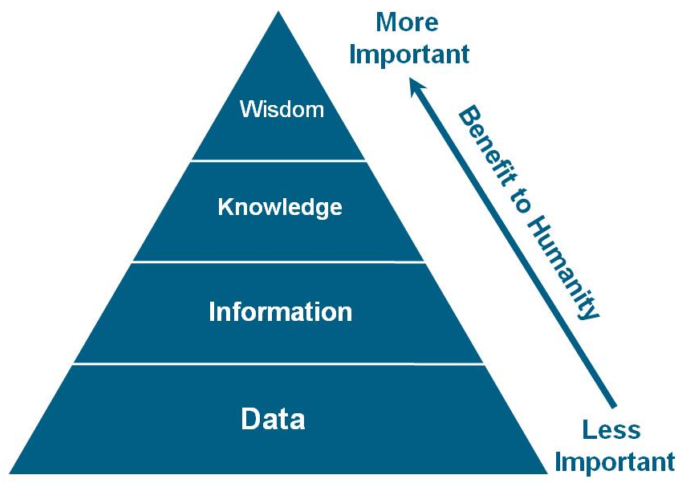
\includegraphics[width=\textwidth]{wkid}
			\fonte{\citetexto{Cisco2011}}
		\end{minipage}
	\end{figure}
	
%TODO Medir & Otimizar (gestão de processos)
	decisoes em tempo real a partir de leituras de sensores
	alta resolução dos dados, possibilitando controle individual de recursos 
	(big data)
	
%TODO Relacionar com Big Data
	
	\citetexto{Cisco2011} estima que em 2015 haverão 25 bilhões de 
	dispositivos conectados a Internet e que apenas 5 anos depois, em 
	2020, este número chegará a casa de 50 bilhões.

\section{Desafios}

%TODO Tecnológicos: bateria, processamento, antenas, protocolos
%TODO Sociais: ética, privacidade (big brother)

\section{Oportunidades}

	IBM Smarter Planet
	HP?
	
	inteligencia por agregação de dados
	processos autonomos
	
	explicar as principais vantagens do uso de IoT nos seguintes contextos
	Industria
	Meio Ambiente
	Sociedade (governamental)
	depois identificar e exemplificar os Application Domains 
	\cite{Sundmaeker2010}


\chapter{Proposta para IoT}

	Abordar neste capítulo as necessidades específicas de IoT e suas 
	características.
	
	Apresentar as dificuldades (problemas) que levarão para as propostas
	de como resolvê-las com as extensões ao protocolo.
	
	
	\section{Multicast}
		
		Propor o uso de multicast para enviar diversos comandos aos objetos
		disponíveis na rede.
		
		
	\section{Tageamento de Objetos}
		
		Propor um sistema para tagear objetos com base em características
		arbitrárias definidas pelo fabricante e pelo usuário.
		
		Quero enviar este comando para todos os objetos elétricos, para
		todos que estão na cozinha, para todos os sensores...
		
		
	\section{Compressão de Headers}
		
		Conforme feito por \cite{Choi2009}
		
		
	\section{Compressão de Dados}
		
		No caso do SNMP compressão das PDUs conforme \cite{Choi2009}
		
		
	% DESPRIORIZAR PORQUE É MUITO IGUAL E IMPORTANTE NO OUTRO ARTIGO
	\section{Requests Periódicos}
		
		Configurar uma mensagem que faz com que os clientes enviem
		dados de forma periódica para o server, evitando a necessidade
		de realizar pooling para obter informações.
		\cite{Choi2009}
		
		
%cronograma revisado
%metodologia revisada
%considerações finais
\chapter{Planejamento da Implementação}

Projetar como vai ser feita a query:
avg(cosumo), 	sala 						> 20 w/h
min(volume), 	quarto sala 				> -5db
estado, 		sala 						> host1:0 host2:1
voltagem, 		gps.lat:21.4 gsp.long:44.3 	> host3:110 host4: 220


\begin{verbatim}
aubinMIB
  - TagManager
    > Listar
    > Adicionar
    > Remover
  - TagDB
    - Tipo
      - Eletrônico
        > Estado (on / off)
        > Voltagem
        > Consumo
      - Áudio
        > Volume
      - Vídeo
        > Width
        > Height
        > Cores
      - Iluminação
        > Luminosidade %
        > Cor
    - Localização
      - GPS
        > Latitude
        > Longitude
      - Domiciliar
        - Sala
        - Quarto
        - Cozinha
\end{verbatim}

Manager precisa saber todas as tags de cada elemento pra conseguir fazer 
consultas por tag. Criar uma "resource" que notifica o manager das alterações 
nas tags (publish/subscribe) do COAP. Senão corre o risco do manager ficar com 
um estado desatualizado / inconsistente.

No caso do COAP os OIDs são traduzidos para resources, podendo ficar do tipo: 

\url{coap://192.168.1.15/snmp/tags/tipo/eletronico/estado}

tais resources recebem comandos RESTful (GET, POST, PUT, DELETE). Por exemplo, 
para desligar e ligar um objeto enviaria um request do tipo:

\url{POST(0) coap://192.168.1.15/snmp/tags/tipo/eletronico/estado}

\url{POST(1) coap://192.168.1.15/snmp/tags/tipo/eletronico/estado}

Adicionalmente, para reduzir o overhead poderia tentar criar um "alias" para 
as resources, tornando duas urls equivalentes, por exemplo:

\url{coap://192.168.1.15/snmp/tags/tipo/eletronico/estado}

\url{coap://192.168.1.15/snmp/tags/2/1/1}

	%TODO cronograma
	
	%TODO Diagrama de blocos entre dispositivos e gerente com as trocas de 
	%mensagens
	
	%TODO Como avaliar: Quantidade / tamanho das mensagens, tempos de 
	%resposta e processamento, consumo de recursos (pouco importante)
	

	Documentar o processo de implementação\ldots
	
	
	
	
%=======================================================================
% Referências
%=======================================================================
%TODO Revisar completeza dos dados
\bibliography{library}


%=======================================================================
% Exemplo de Apêndice
% O Apêndice é utilizado para apresentar material complementar elaborado
% pelo próprio autor.  Deve seguir as mesmas regras de formatação do
% corpo principal do documento.
%=======================================================================
%\appendix
%\chapter{Informações Complementares}
%
%O Apêndice é utilizado para apresentar material complementar elaborado
%pelo próprio autor.  Deve seguir as mesmas regras de formatação do
%corpo principal do documento.


%=======================================================================
% Exemplo de Anexo
% O Anexo é utilizado para a ``inclusão de materiais não elaborados pelo
% próprio autor, como cópias de artigos, manuais, folders, balancetes, etc.
% e não precisam estar em conformidade com o modelo''.
%=======================================================================
%\annex
%\chapter{Artigos Publicados}
%
%O Anexo é utilizado para a ``inclusão de materiais não elaborados pelo
%próprio autor, como cópias de artigos, manuais, folders, balancetes, etc.
%e não precisam estar em conformidade com o modelo''.


\end{document}
